\documentclass[8pt,a4paper,compress,handout]{beamer}

\usepackage{/home/siyer/lib/slides}

\title{Algorithms and Data Structures}
\date{}

\begin{document}
\begin{frame}
\vfill
\titlepage
\end{frame}

\begin{frame}
\frametitle{Outline}
\tableofcontents
\end{frame}

\section{Performance}
\begin{frame}[fragile]
\emph{Algorithms} are methods for solving computational problems.

\bigskip

\emph{Data structures} are schemes for arranging data, amenable to efficient processing by algorithms.

\bigskip

The performance characteristics of a program is determined by: 
\begin{itemize}
\item its \emph{time complexity}, ie, how long it takes; and 

\item its \emph{space complexity}, ie, how much memory it needs.
\end{itemize}
\end{frame}

\begin{frame}[fragile]
The running time of a program is determined by the cost of executing each statement, and the frequency of execution of each statement.

\bigskip

Running time is expressed using an \emph{order-of-growth} function of the problem size $N$, without any lower-order terms or constant coefficients.

\bigskip

Order-of-growth classifications:
\begin{center}
\begin{tabular}{cccc}
description & function & code description & example \\ \hline
constant & 1 & statement & add two numbers \\
logarithmic & $\log N$ & divide in half & binary search \\
linear & $N$ & loop & find the maximum \\
linearithmic & $N\log N$ & divide and conquer & merge sort \\
quadratic & $N^2$ & double loop & check all pairs \\
cubic & $N^3$ & triple loop & check all triples \\
exponential & $2^N$ & exhaustive search & check all subsets
\end{tabular} 
\end{center}
\begin{center}
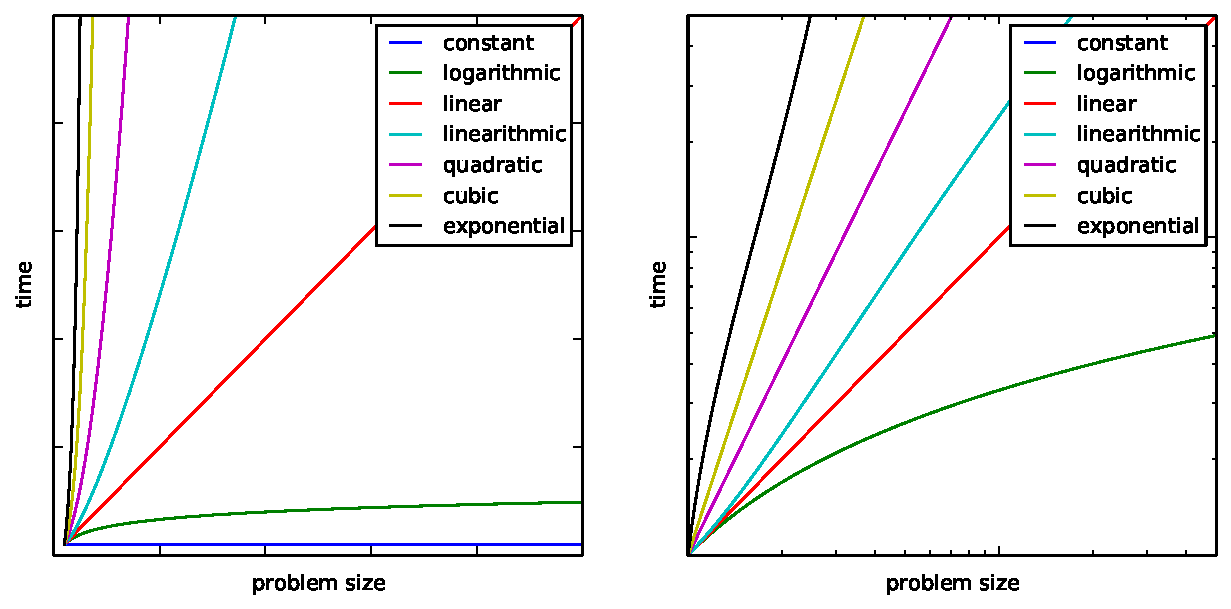
\includegraphics[scale=0.25]{{./figures/order_of_growth}.pdf}
\end{center}
\end{frame}

\begin{frame}[fragile]
The sizes of objects of built-in types differ from system to system, so the sizes of data types that we create also differ accordingly.

\bigskip

The function call \lstinline{sys.getsizeof(x)} returns the number of bytes that a built-in object \lstinline{x} consumes on a particular system.

\bigskip

Sizes of built-in objects on a typical system:
\begin{center}
\begin{tabular}{cc}
object & size in bytes \\ \hline
integer & 24 \\ 
float & 24 \\ 
boolean & 24 \\ 
string of $n$ characters & $40 + n$ \\
list of $n$ integers & $72 + 8n + 24n = 72 + 32n$ \\
$m$-by-$n$ list of integers & $72 + 8m + m(72 + 32n) = 72 + 80m + 32mn$ \\
user-defined & hundreds of bytes, at least
\end{tabular} 
\end{center}
\end{frame}

\section{Searching}
\begin{frame}[fragile]
The \emph{search problem} involves searching for a key in a collection of $N$ keys.

\bigskip

Linear search:
\begin{lstlisting}[language=Python]
def search(key, a):
    for i, v in enumerate(a):
        if key == v:
            return i
    return -1
\end{lstlisting}

\bigskip

Binary search:

\begin{minipage}{150pt}
\begin{center}
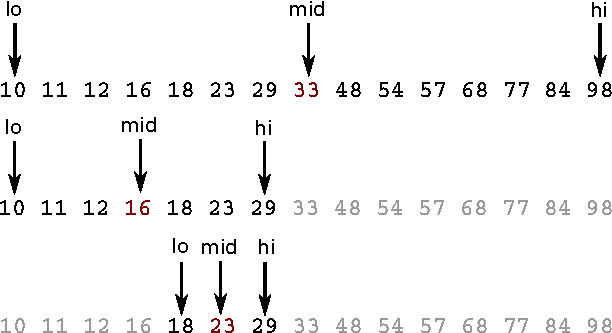
\includegraphics[scale=0.4]{./figures/bs1.pdf}

\smallskip

\tiny successful search for the key 23
\end{center}
\end{minipage}
\begin{minipage}{150pt}%
\hfill
\begin{center}
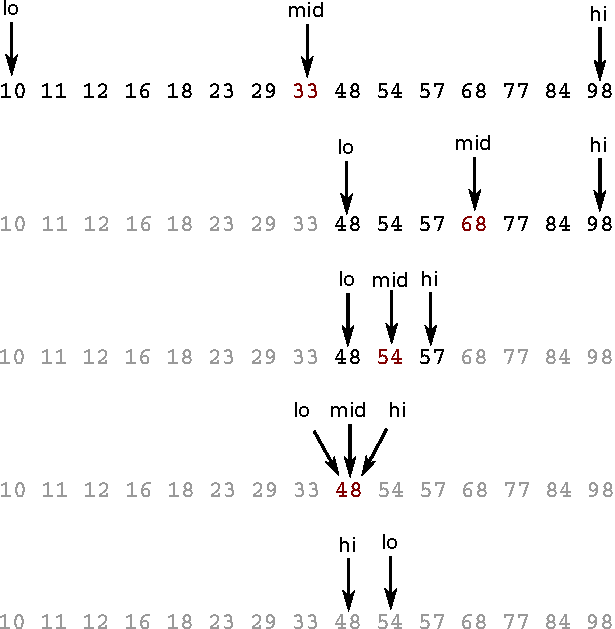
\includegraphics[scale=0.4]{./figures/bs2.pdf}

\smallskip

\tiny unsuccessful search for the key 50
\end{center}
\end{minipage}
\end{frame}

\begin{frame}[fragile]
\begin{framed}
\tiny \lstinline{binarysearch.py}: Accepts as a command-line argument a string which is the name of a whitelist file, and writes to standard output the keys in standard input that are not in the whitelist file.
\end{framed}

\begin{lstlisting}[language=Python]
import instream
import stdio
import sys

def _search(key, a, lo, hi):
    if hi <= lo:
        return -1
    mid = (lo + hi) // 2
    if key < a[mid]:
        return _search(key, a, lo, mid)
    elif a[mid] < key:
        return _search(key, a, mid + 1, hi)
    else:
        return mid

def search(key, a):
    return _search(key, a, 0, len(a))

def main():
    inStream = instream.InStream(sys.argv[1])
    a = inStream.readAllStrings()
    while not stdio.isEmpty():
        key = stdio.readString()
        if search(key, a) < 0:
            stdio.writeln(key)

if __name__ == '__main__':
    main()
\end{lstlisting}
\end{frame}

\begin{frame}[fragile]
\begin{lstlisting}[language={}]
$ more emails.txt 
bob@office
carl@beach
marvin@spam
bob@office
bob@office
mallory@spam
dave@boat
eve@airport
alice@home
\end{lstlisting}

\begin{lstlisting}[language={}]
$ more white.txt
alice@home
bob@office
carl@beach
dave@boat
\end{lstlisting}

\begin{lstlisting}[language={}]
$ python binarysearch.py white.txt < emails.txt 
marvin@spam
mallory@spam
eve@airport
\end{lstlisting}
\end{frame}

\section{Sorting}
\begin{frame}[fragile]
The \emph{sort problem} involves rearranging a sequence of objects so as to put them in some logical order.

\bigskip

\emph{Insertion sort} is similar to sorting a bridge hand --- consider the cards one at a time, inserting each into its proper place among those already considered.
\begin{center}
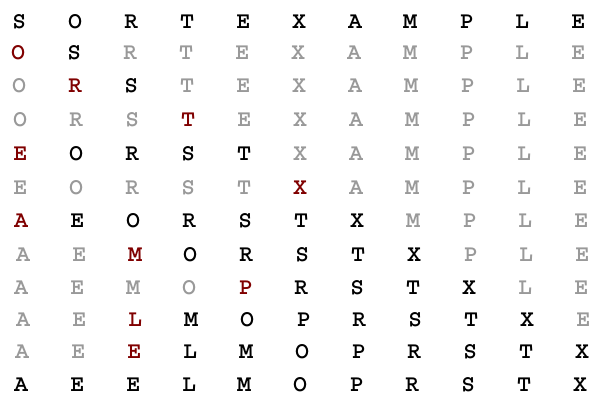
\includegraphics[scale=0.3]{figures/insertion.png}

\smallskip

\tiny insertion sort
\end{center}
\end{frame}

\begin{frame}[fragile]
\begin{framed}
\tiny \lstinline{insertion.py}: Reads strings from standard input, sorts them into increasing order, and writes them to standard output.
\end{framed}

\begin{lstlisting}[language=Python]
import stdio
import sys

def exchange(a, i, j):
    a[i], a[j] = a[j], a[i]

def sort(a):
    n = len(a)
    for i in range(1, n):
        j = i
        while (j > 0) and (a[j] < a[j - 1]):
            exchange(a, j - 1, j)
            j -= 1

def main():
    a = stdio.readAllStrings()
    sort(a)
    for s in a:
        stdio.write(s + ' ')
    stdio.writeln()

if __name__ == '__main__':
    main()
\end{lstlisting}

\begin{lstlisting}[language={}]
$ more tiny.txt 
the and was his you tom but for had him
\end{lstlisting}

\begin{lstlisting}[language={}]
$ python insertion.py < tiny.txt 
and but for had him his the tom was you 
\end{lstlisting}
\end{frame}

\begin{frame}[fragile]
\emph{Merge sort} is based on a simple operation known as \emph{merging}: combining two ordered lists to make one larger ordered list.

\bigskip

To sort a list, we divide it into two halves, sort the two halves recursively, and then merge the results.

\begin{center}
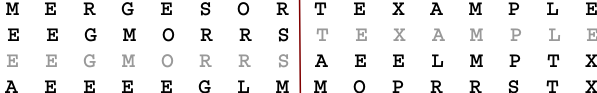
\includegraphics[scale=0.3]{figures/merge.png}

\smallskip

\tiny merge sort
\end{center}
\end{frame}

\begin{frame}[fragile]
\begin{framed}
\tiny \lstinline{merge.py}: Reads strings from standard input, sorts them into increasing order, and writes them to standard output.
\end{framed}

\begin{lstlisting}[language=Python]
import stdarray
import stdio
import sys

def _merge(a, lo, mid, hi, aux):
    n = hi - lo
    i = lo
    j = mid
    for k in range(n):
        if i == mid:
            aux[k] = a[j]
            j += 1
        elif j == hi:
            aux[k] = a[i]
            i += 1
        elif a[j] < a[i]:
            aux[k] = a[j]
            j += 1
        else:
            aux[k] = a[i]
            i += 1
    a[lo:hi] = aux[0:n]
\end{lstlisting}
\end{frame}

\begin{frame}[fragile]
\begin{lstlisting}[language=Python]
def _sort(a, lo, hi, aux):
    n = hi - lo
    if n <= 1:
        return
    mid = (lo + hi) // 2
    _sort(a, lo, mid, aux)
    _sort(a, mid, hi, aux)
    _merge(a, lo, mid, hi, aux)

def sort(a):
    n = len(a)
    aux = stdarray.create1D(n)
    _sort(a, 0, n, aux)

def main():
    a = stdio.readAllStrings()
    sort(a)
    for s in a:
        stdio.write(s + ' ')
    stdio.writeln()

if __name__ == '__main__':
    main()
\end{lstlisting}

\begin{lstlisting}[language={}]
$ more tiny.txt 
the and was his you tom but for had him
\end{lstlisting}

\begin{lstlisting}[language={}]
$ python merge.py < tiny.txt 
and but for had him his the tom was you 
\end{lstlisting}
\end{frame}

\begin{frame}[fragile]
\begin{framed}
\tiny \lstinline{frequencycount.py}: Reads words from standard input, and writes the frequency counts of the words to standard output.
\end{framed}

\begin{lstlisting}[language=Python]
import stdio
import sys
from counter import Counter

def main():
    words = stdio.readAllStrings()
    words.sort()
    zipf = []
    for i in range(len(words)):
        if (i == 0) or (words[i] != words[i - 1]):
            entry = Counter(words[i], len(words))
            zipf += [entry]
        zipf[len(zipf) - 1].increment()
    zipf.sort()
    zipf.reverse()
    for entry in zipf:
        stdio.writeln(entry)

if __name__ == '__main__':
    main()
\end{lstlisting}

\begin{lstlisting}[language={}]
$ python frequencycount.py < tomsawyer.txt
the: 3452
and: 2908
a: 1758
to: 1741
of: 1539
was: 1124
in: 926
...
\end{lstlisting}
\end{frame}

\section{Stacks}
\begin{frame}[fragile]
A \emph{stack} is an iterable collection that is based on the last-in-first-out (LIFO) policy.

\bigskip

A data type \lstinline{Stack} that represents a stack:
\begin{center}
\begin{tabular}{cc}
method & description \\ \hline
\lstinline$Stack()$ & constructs an empty stack $s$ \\
\lstinline$s.isEmpty()$ & tests if $s$ empty \\
\lstinline$s.push(item)$ & pushes $item$ on top of $s$ \\
\lstinline$s.pop()$ &  pops and returns the item on top of $s$ \\
\lstinline$str(s)$ & returns a string representation of $s$
\end{tabular} 
\end{center}
\end{frame}

\begin{frame}[fragile]
\begin{framed}
\tiny \lstinline{stack.py}: Defines a data type \lstinline{Stack}.
\end{framed}

\begin{lstlisting}[language=Python]
import stdio

class Stack:
    def __init__(self):
        self._a = []

    def isEmpty(self):
        return len(self._a) == 0

    def push(self, item):
        self._a += [item]

    def pop(self):
        return self._a.pop()

    def __str__(self):
        s = ''
        for item in self._a:
            s = str(item) + ' ' + s
        return s
\end{lstlisting}
\end{frame}

\begin{frame}[fragile]
\begin{lstlisting}[language=Python]
def main():
    stack = Stack()
    while not stdio.isEmpty():
        item = stdio.readString()
        if item != '-':
            stack.push(item)
        else:
            stdio.write(stack.pop() + ' ')
    stdio.writeln()

if __name__ == '__main__':
    main()
\end{lstlisting}

\begin{lstlisting}[language={}]
$ more tobe.txt
to be or not to - be - - that - - - is
\end{lstlisting}

\begin{lstlisting}[language={}]
$ python stack.py < tobe.txt 
to be not that or be
\end{lstlisting}
\end{frame}

\begin{frame}[fragile]
\begin{framed}
\tiny \lstinline{evaluate.py}: Reads a fully parenthesized numeric expression from standard input, evaluates it, and writes the resulting number to standard output.
\end{framed}

\begin{lstlisting}[language=Python]
import math
import stdio
from stack import Stack

def main():
    ops, values = Stack(), Stack()
    while not stdio.isEmpty():
        token = stdio.readString()
        if   token == '+':    ops.push(token)
        elif token == '-':    ops.push(token)
        elif token == '*':    ops.push(token)
        elif token == 'sqrt': ops.push(token)
        elif token == ')':
            op, value = ops.pop(), ops.pop()
            if   op == '+':    value = values.pop() + value
            elif op == '-':    value = values.pop() - value
            elif op == '*':    value = values.pop() * value
            elif op == 'sqrt': value = math.sqrt(value)
            values.push(value)
        elif token != '(':
            values.push(float(token))
    stdio.writeln(values.pop())

if __name__ == '__main__':
    main()
\end{lstlisting}

\begin{lstlisting}[language={}]
$ python evaluate.py
( ( 1 + sqrt ( 5.0 ) ) * 0.5 )
<ctrl-d>
1.61803398875
\end{lstlisting}
\end{frame}

\section{Queues}
\begin{frame}[fragile]
A \emph{queue} is an iterable collection that is based on the first-in-first-out (FIFO) policy.

\bigskip

A data type \lstinline{Queue} that represents a queue:
\begin{center}
\begin{tabular}{cc}
method & description \\ \hline
\lstinline$Queue()$ & constructs an empty queue $q$ \\
\lstinline$q.isEmpty()$ & tests if $q$ empty \\
\lstinline$q.enqueue(item)$ & adds $item$ to the end of $q$ \\
\lstinline$q.dequeue()$ &  removes and returns the first item of $q$ \\
\lstinline$str(q)$ & returns a string representation of $q$
\end{tabular} 
\end{center}
\end{frame}

\begin{frame}[fragile]
\begin{framed}
\tiny \lstinline{queue.py}: Defines a data type \lstinline{Queue}.
\end{framed}

\begin{lstlisting}[language=Python]
import stdio

class Queue:
    def __init__(self):
        self._a = []

    def isEmpty(self):
        return len(self._a) == 0

    def enqueue(self, item):
        self._a.insert(0, item)

    def dequeue(self):
        return self._a.pop()

    def __str__(self):
        s = ''
        for item in reversed(self._a):
            s = s + ' ' + str(item)
        return s
\end{lstlisting}
\end{frame}

\begin{frame}[fragile]
\begin{lstlisting}[language=Python]
def main():
    queue = Queue()
    while not stdio.isEmpty():
        item = stdio.readString()
        if item != '-':
            queue.enqueue(item)
        else:
            stdio.write(queue.dequeue())
            stdio.write(' ')
    stdio.writeln()

if __name__ == '__main__':
    main()
\end{lstlisting}

\begin{lstlisting}[language={}]
$ more tobe.txt
to be or not to - be - - that - - - is
\end{lstlisting}

\begin{lstlisting}[language={}]
$ python queue.py < tobe.txt
to be or not to be
\end{lstlisting}
\end{frame}

\begin{frame}[fragile]
\begin{framed}
\tiny \lstinline{mm1queue.py}: Accepts float command-line arguments \carg{lamb} and \carg{mu}, simulates an M/M/1 queue with arrival rate \carg{lamb} and service rate \carg{mu}.
\end{framed}

\begin{lstlisting}[language=Python]
import stddraw
import stdrandom
import sys
from histogram import Histogram
from queue import Queue

def main():
    lamb, mu = float(sys.argv[1]), float(sys.argv[2])
    histogram = Histogram(60 + 1)
    queue = Queue()
    stddraw.setCanvasSize(700, 500)
    nextArrival = stdrandom.exp(lamb)
    nextService = nextArrival + stdrandom.exp(mu) 
    while True:
        while nextArrival < nextService:
            queue.enqueue(nextArrival)
            nextArrival += stdrandom.exp(lamb)
        arrival = queue.dequeue()
        wait = nextService - arrival
        stddraw.clear()
        histogram.addDataPoint(min(60, int(round(wait))))
        histogram.draw()
        stddraw.show(20.0)
        if queue.isEmpty():
            nextService = nextArrival + stdrandom.exp(mu)
        else:
            nextService = nextService + stdrandom.exp(mu)

if __name__ == '__main__':
    main()

\end{lstlisting}
\end{frame}

\begin{frame}[fragile]
\begin{minipage}{200pt}
\begin{lstlisting}[language={}]
$ python mm1queue.py .167 .25
\end{lstlisting}
\end{minipage}%
\hfill
\begin{minipage}{100pt}
\begin{center}
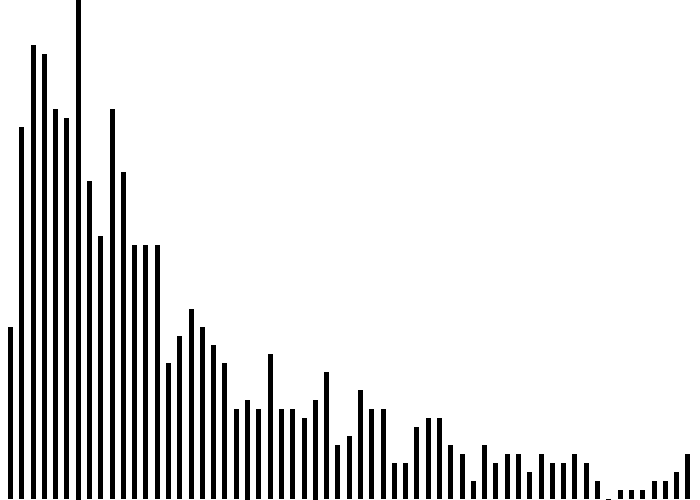
\includegraphics[scale=0.15]{figures/mm1queue1.png}

\smallskip

\tiny M/M/1 queue ($\lambda=0.167, \mu=0.25$)
\end{center}
\end{minipage}%

\bigskip

\begin{minipage}{200pt}
\begin{lstlisting}[language={}]
$ python mm1queue.py .167 .2
\end{lstlisting}
\end{minipage}%
\hfill
\begin{minipage}{100pt}
\begin{center}
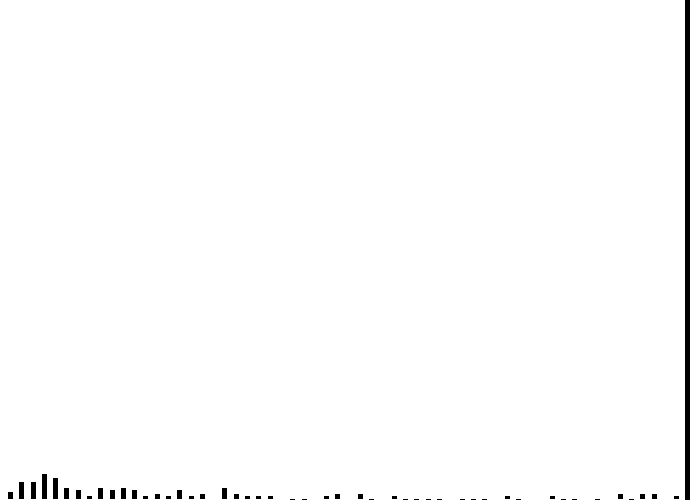
\includegraphics[scale=0.15]{figures/mm1queue2.png}

\smallskip

\tiny M/M/1 queue ($\lambda=0.167, \mu=0.2$)
\end{center}
\end{minipage}
\end{frame}
\end{document}
